\section{Autismo}

L'autismo è una patologia complessa, che oggi si ritiene essere in
vorticoso aumento. Per la stranezza del quadro clinico e per altri
motivi, la comunità scientifica negli ultimi 10 anni ha sviluppato un
grande interesse per questa patologia.

\subsection{Definizione}

Con il termine autismo ci riferiamo a un vario e variabile numero di
quadri patologici che nel loro insieme definiscono un continuum da forme
più leggere, sfumate, anche clinicamente difficili da inquadrare, a
forme più gravi: questi oggi vengono definiti \textbf{disturbi dello
``spettro autistico'' (DSA)}.

Sono un insieme di quadri che hanno in comune la compromissione delle
aree:

\begin{itemize}
\item
  della comunicazione (non solo il linguaggio verbale, anche quello del
  corpo)
\item
  delle capacità sociali
\item
  della capacità di fare esperienze e di condividerle
\item
  di molte altre funzioni.
\end{itemize}

La conseguenza di questo è una \textbf{compromissione estremamente
varia} di tutto il funzionamento della persona che appare strana e
bizzarra, ai nostri occhi incomprensibile, \textbf{e} \textbf{pervasiva}
perché non c'è funzione che, in misura maggiore o minore, in qualche
modo non sia interessata da questa. Il risultato finale è un'alterazione
pesantissima della vita sociale e della cognizione sociale.
\\\\
Ma che cos'è la cognizione sociale? È quella serie di contenuti mentali
che ci consente di adattarci all'ambiente in cui viviamo, di capirne le
regole, i condizionamenti, in definitiva l'ampia articolazione di tutto
quello che ci circonda; ci sono cose che in alcuni contesti sono lecite,
in altri no; una serie di regole e norme sociali che hanno a che fare
col senso comune e non solo con l'educazione.
\\\\
Nonostante il termine autismo indichi soltanto una delle manifestazioni
dello ``spettro autistico'', viene usato come se i vari quadri presenti
in questo spettro fossero equivalenti. In realtà non è cosi perché i
funzionamenti sono estremamente diversi: possiamo incontrare persone con
DSA estremamente intelligenti, geniali, sino a persone molto povere dal
punto di vista cognitivo (come da alcuni veniva definito ``ritardo
mentale grave'') con anche assenza di linguaggio, persone con cui è
veramente difficile intendersi.

Quindi questo spettro è come un grande ombrello sotto cui troviamo
espressioni fenotipiche le più disparate e diverse.

\subsection{Storia}

L'autismo veniva in origine definito ``autismo infantile'', termine
coniato da Kanner nel 1942, preso da Bloiler (psicanalista contemporaneo
di Freud), il quale aveva applicato questo termine ``autistico'' al
distacco dalla realtà (distacco emotivo, bisogno di isolamento) che era
caratteristico del paziente schizofrenico, soprattutto con
sintomatologia negativa.

Kanner identificò bambini che erano accomunati da questo bisogno di
starsene per proprio conto (tipico atteggiamento di chi ignora il
mondo), e nei quali non era presente il linguaggio.

Egli ritenne che la patologia fosse dovuta a un fatto relazionale
determinato dalla ``freddezza'' del rapporto che i genitori
intrattenevano col bambino, soprattutto da parte della madre (``madri
frigorifero'', così chiamate da Bettelheim).

Dunque fino agli anni '70 l'autismo, riconosciuto solo come autismo
infantile, veniva considerato una \textbf{psicosi}.
\\\\
Dagli anni '80 in poi nei manuali diagnostici (come il DSM IV, l'odierno
DSM 5, l'ICD 10) scompare l'aggettivo ``infantile'', alludendo alla
durata life-long, e quindi al concetto di \textbf{cronicità} e
all'\textbf{origine} \textbf{biologica} (C'è sempre stata una disputa in
ambito psichiatrico tra i sostenitori delle teorie biologiche e quelli
delle teorie psicodinamiche-psicanalitiche; prima avevano il primato
queste ultime, oggi la tendenza è invertita).

Nel DSM IV di allora (che denominava tutte questi disturbi non DSA ma
``disturbi pervasivi dello sviluppo'', DPS) venivano individuate 5
categorie sottodiagnostiche:

\begin{itemize}
\item
  \textbf{autismo propriamente detto}
\item
  \textbf{sindrome di Rett:} l'unica tra questi quadri ad avere una vera
  linea genetica. Colpisce solo le femmine, presenta una pesante di
  compromissione neurologica, ad andamento ingravescente
\item
  \textbf{disturbo disintegrativo dell'infanzia:} la psicosi infantile
  sostanzialmente. Ha la caratteristica di comparire tra i 3-5 anni, è
  pesante perché non si vedono miglioramenti con la crescita, anzi
  spesso questi bambini accompagnano un deficit cognitivo importante
\item
  \textbf{sindrome di Asperger:} più o meno in contemporanea con Kanner,
  Asperger a Vienna individuò alcuni bambini con caratteristiche simili
  a quelle dei bambini studiati da Kanner, ma al contrario di quelli
  avevano un'intelligenza spiccatissima e parlavano; avevano in comune
  un disinteresse, talvolta totale, per il mondo circostante e per gli
  altri: le altre persone, gli altri bambini non rappresentano categorie
  interessanti -- né per gli autistici propriamente detti, né per gli
  Asperger. Ricordate degli Asperger che hanno un funzionamento
  cognitivo normale o molto elevato.
\item
  \textbf{PDD NOS} (disturbi pervasivi dello sviluppo non altrimenti
  specificati): una serie di disturbi con molte caratteristiche in
  comune con l'autismo; il quadro clinico può non essere completo, il
  linguaggio indipendentemente dalle situazioni può essere presente o
  meno, alcuni sono abili dal punto di vista motorio, altri non lo sono;
  in linea di massima si tratta di forme più sfumate.
\end{itemize}

Nel DSM 5, a differenza del DSM IV che prendeva in considerazione
soltanto il comportamento e i quadri clinici determinati da questi,
quindi una classificazione di tipo \textbf{categoriale}, senza
riferimenti alla gravità, nel DSM 5 viene perso in considerazione in
livello di gravità, si parla di forme gravi, medie, lievi, sfumate di
DSA, c'è quindi un tentativo di approccio \textbf{dimensionale}. Vengono
eliminate le sottocategorie diagnostiche: tutto è spettro autistico,
dalla forma gravissima al genio Asperger.

Le novità del DSM 5 importanti sono che questi disturbi non rientrano
più nella categoria dei disturbi mentali ma l'autismo viene ora definito
un disturbo del neurosviluppo. Viene dato poi molto rilievo alle
anomalie sensoriali (vedi poi).

Problemi del nuovo modello:

\begin{itemize}
\item
  Più enfasi al criterio puramente comportamentale e scarso spazio alla
  riflessione psicopatologica, alla riflessione clinica
\item
  L'esperienza soggettiva del malato, cioè come il paziente vive il
  proprio disturbo, e la sua storia vengono trascurate
\item
  Criterio diagnostico molto uniformante, con scarsa attenzione alle
  differenziazioni (si va infatti dal genio al soggetto che non
  comprende proprio nulla).
\end{itemize}

\subsection{Epidemiologia}

Molto più frequente nei maschi che nelle femmine, rapporto 4:1.

Non ci sono differenziazioni etniche o socioculturali (Kanner era invece
convinto che i bambini autistici appartenessero tutti a ceti abbienti).

Negli ultimi anni c'è stato un incremento pazzesco, qualcuno ha parlato
di ``epidemia dell'autismo''. I dati di prevalenza sono discordanti, da
20-25/10.000 a 1/67 bambini (una follia); in Emilia-Romagna più o meno
6/1000. Importante è che non è più considerato patologia rara.
Considerate che i dati di prevalenza dipendono anche dai criteri di
inclusione diagnostica: se vedo un bambino ben funzionante un po'
strano, con difficoltà di relazione coi pari, dirò che ha dei
\emph{tratti} di DSA, qualche altro collega potrebbe invece così
classificarlo.
\\\\
L'incremento della patologia autistica negli ultimi 11 anni è del 805\%,
a fronte del 31\% di disabilità in senso generale.

Le possibili cause dell'aumento:

\begin{itemize}
\item
  iperinclusione diagnostica
\item
  più conosciuto, meglio diagnosticato
\item
  grande interesse della comunità scientifica
\item
  tutti i disturbi mentali sono in aumento, soprattutto in età evolutiva
  (bambini e adolescenti)
\item
  rapidi cambiamenti a cui è sottoposta la nostra società possono
  slatentizzare una certa vulnerabilità rispetto alla capacità di
  acquisire la cognizione sociale
\item
  interesse di ``big business'' (forse anche per questo lo si
  diagnostica così facilmente).
\end{itemize}

Non abbiamo dati di adulti autistici perché è una diagnosi che tende a
scomparire dall'età infantile a quella adulta - forse sempre perché non
è ancora ben conosciuta. Anche quando viene fatto il passaggio dai
servizi per l'età evolutiva ai servizi per l'età adulta, non compare più
la parola ``autismo'' ma diventano ``persone con ritardo mentale'' o
vengono classificati come ``esiti di psicosi infantile''.

\subsection{Clinica}

Quello che vediamo nella persona autistica è legato ad anomalie presenti
nei seguenti domini:

\begin{itemize}
\item
  \textbf{interazione sociale reciproca} (importante il ``reciproco'':
  posso interagire con chiunque anche senza che ci sia reciprocità di
  azione, senza quindi uno scambio)
\item
  \textbf{capacità di condividere idee e sentimenti} (la comprensione di
  idee e sentimenti degli altri sono una cosa inesistente per i soggetti
  autistici, anche quelli molto intelligenti! Non riescono a mettersi
  nei panni dell'altro, è impossibile condividere alcunché)
\item
  \textbf{cognizione sociale}
\item
  \textbf{rigidità cognitiva} (caratteristica tipica dell'autismo ma che
  non appartiene esclusivamente a questa categoria, si ritrova anche in
  disturbi della personalità. Anche qui indipendentemente dal
  funzionamento)
\end{itemize}

analizziamo nel dettaglio:

\begin{figure}[!ht]
\centering
	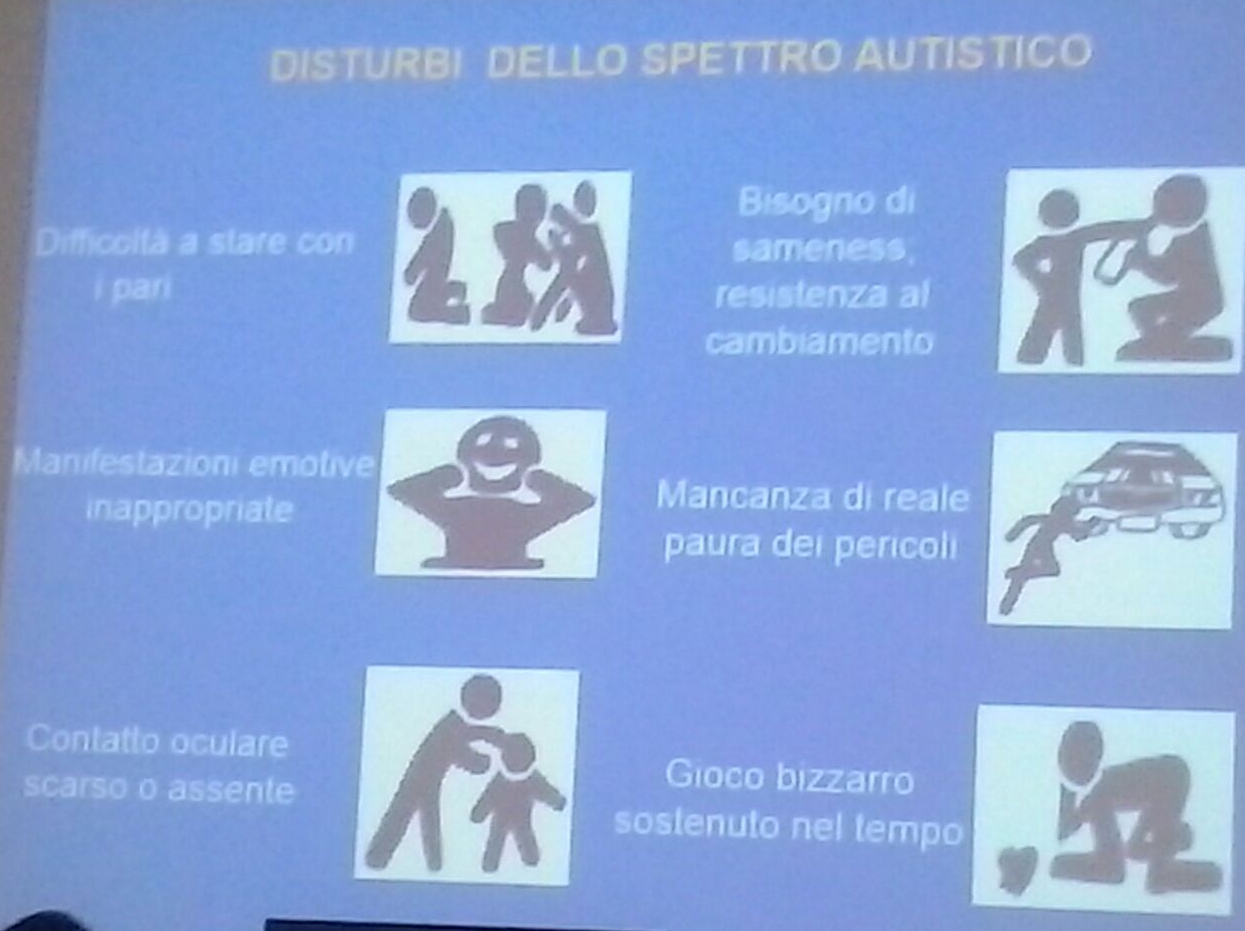
\includegraphics[width=0.9\textwidth]{014/image1.png}
\end{figure}

\begin{itemize}
\item[1.]
  \textbf{difficoltà a stare con i pari.} Classicamente si vede un
  bambino al nido/alla materna/alle elementari in disparte, talvolta
  questo bisogno diventa proprio fisico di allontanamento; girano su se
  stessi, si incantano davanti alla finestra, tormentano un lembo di
  tessuto, strappano le pagine di un libro -- non per fare un dispetto
  ma perché la consistenza della carta e il rumore della carta strappata
  rientrano nell'autosensorilità (vedi poi)
\item[2.]
  \textbf{manifestazioni emotive inappropriate.} Molto frequente di
  fronte a qualcosa che li disturba, che fa male in senso lato, loro si
  portano le mani alle orecchie. Può essere che abbiano visto una
  persona, o che hanno cambiato strada (non tollerano i cambiamenti), o
  che si da da mangiare un cibo di consistenza diversa da quella a cui
  sono abituati. Il gesto è proprio quello di strizzare le palpebre,
  tapparsi le orecchie come per dire ``non voglio né vedere né
  sentire''. A volte ci sono pianti immotivati, disperati, angosciati,
  noi non capiamo perché ma andando a indagare con domande ai genitori
  una causa si trova sempre
\item[3.]
  \textbf{contatto oculare scarso o assente.} Caratteristica lampante:
  fanno fatica a guardare negli occhi, o magari hanno solo un contatto
  fugace. Talvolta ci sono autistici, anche gravi, che guardano negli
  occhi. In linea di massima il contatto oculare proprio non c'è
\item[4.]
  \textbf{bisogno di sameness (immutabilità), resistenza al
  cambiamento.} I cambiamenti scatenano crisi pazzesche di agitazione,
  difficili da gestire.
\item[5.]
  \textbf{Mancanza di reale paura del pericolo}. Ad esempio lasciano la
  mano e attraversano la strada senza guardare a destra e a sinistra, si
  avvicinano a situazioni pericolose o, anche per quelli molto
  intelligenti, tendono a fidarsi ciecamente degli altri (anche perché
  non sentono la mancanza della presenza della figura di riferimento --
  uno dei segni tipici del sospetto diagnostico nei bambini molto
  piccoli è che vanno in braccio a chiunque in maniera totalmente
  indifferente, e quando la mamma li porta all'asilo è impossibile che
  piangono, tant'è che riteniamo un grande successo quando invece un
  giorno la mamma va via e il bambino piange)
\item[6.]
  \textbf{gioco bizzarro sostenuto nel tempo}: fissare una macchinina,
  metterle in fila, scomporle e rimetterle in fila (nell'adulto ci sono
  attività altrettanto ripetitive ma adeguate all'età)
\end{itemize}

\begin{figure}[!ht]
\centering
	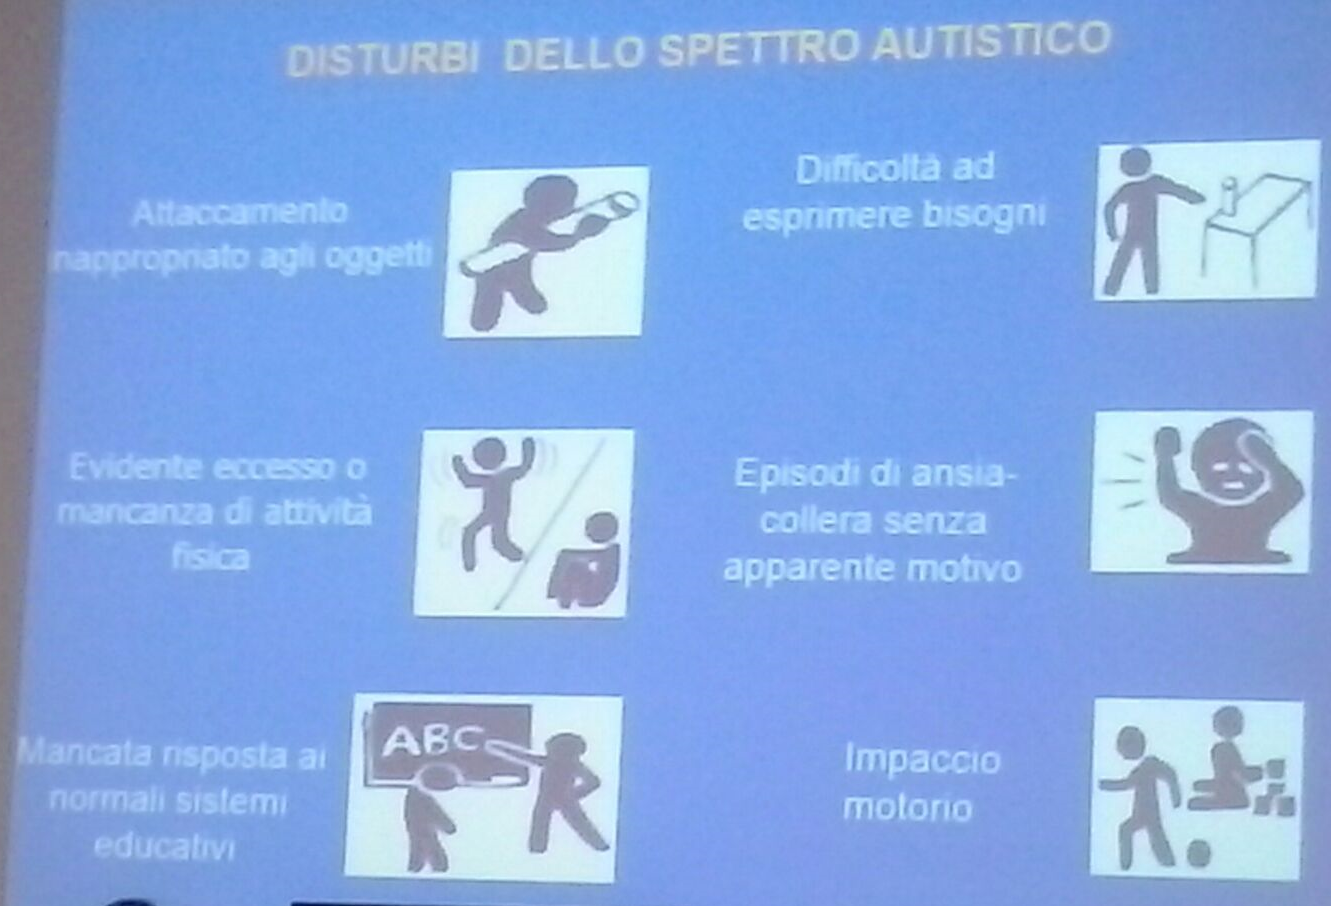
\includegraphics[width=0.9\textwidth]{014/image2.png}
\end{figure}

\begin{itemize}
\item[1.]
  \textbf{attaccamento inappropriato agli oggetti}: anche perché
  preferiscono di gran lunga gli oggetti alle persone. Ci sono poi degli
  oggetti a cui sono particolarmente legati, il cosiddetto ``oggetto
  autistico'' che può essere qualsiasi cosa, anche un pezzetto di legno.
  Tendono a preferire gli oggetti duri rispetto a quelli morbidi
\item[2.]
  \textbf{evidente eccesso o mancanza di attività fisica}: ipoattività o
  iperattività motoria
\item[3.]
  \textbf{mancata risposta ai normali sistemi educativi.} Non capiscono
  le richieste, e questo non è legato al livello di intelligenza ma alla
  percezione di quello che sentono e che vedono; probabilmente questo è
  dovuto a una mancata integrazione di questi stimoli a livello del SNC
\item[4.]
  \textbf{difficoltà ad esprimere bisogni}
\item[5.]
  \textbf{episodi di ansia/collera senza apparente motivo.} Noi non
  capiamo, può essere un cambiamento (esempio di una bambina che a
  scuola verso la fine del pranzo, in mensa, faceva crisi pazzesche, si
  disperava, si buttava per terra; per un anno educatori, insegnanti e
  genitori non hanno capito perché; poi si è scoperto che in quella
  scuola davano solitamente mele gialle, lei invece era abituata, a
  casa, a mangiare mele rosse)
\item[6.]
  \textbf{impaccio motorio.} Tipico soprattutto degli Asperger, mentre
  il bambino autistico grave è abilissimo dal punto di vista motorio
\end{itemize}

\begin{figure}[!ht]
\centering
	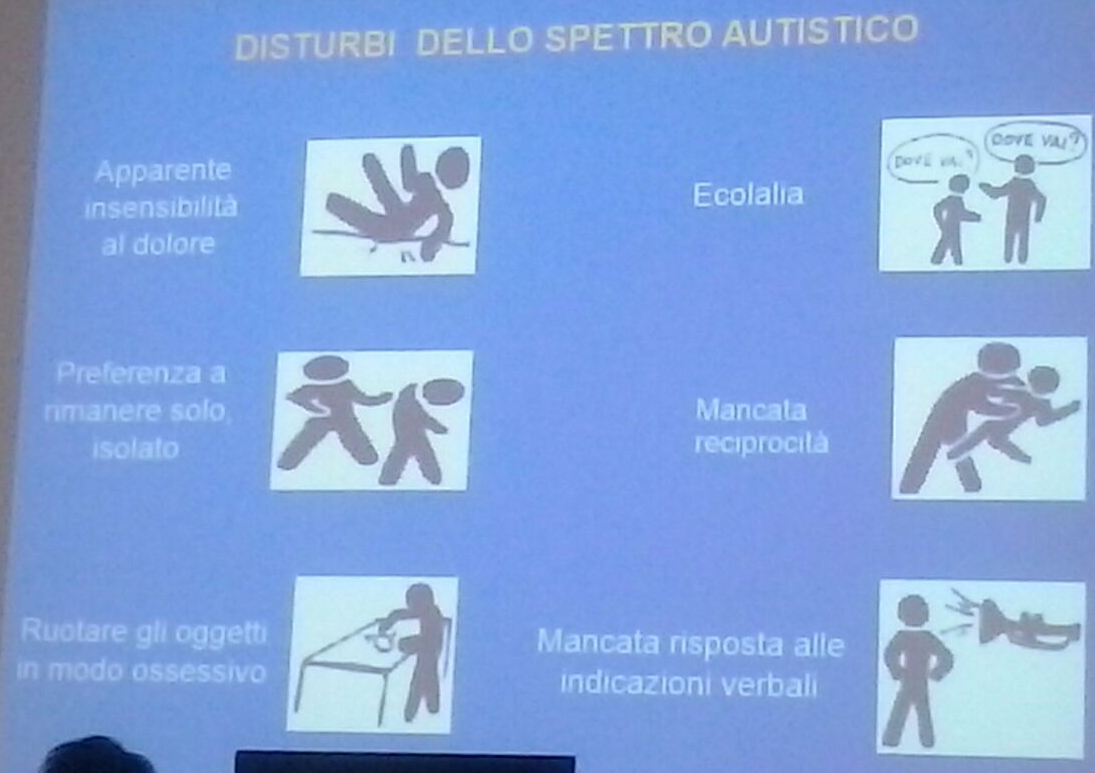
\includegraphics[width=0.9\textwidth]{014/image3.png}
\end{figure}

\begin{itemize}
\item[1.]
  \textbf{apparente insensibilità al dolore, alle temperature}. Se
  cadono non piangono, se si scottano non piangono
\item[2.]
  \textbf{preferenza a rimanere solo, isolato}
\item[3.]
  \textbf{ruotare gli oggetti in modo ossessivo}. Particolare
  predilezione, probabilmente legato all'auto-sensorialità (è qualche
  cosa che parte da uno stimolo sensoriale e attraverso cui riusciamo a
  produrre/riprodurre delle sensazioni piacevoli ma in maniera
  indiretta: esempio il vezzo di arricciarsi una ciocca di capelli può
  essere legata alla concentrazione, al rilassamento o può anche essere
  banalmente piacevole, ha a che fare con l'auto-sensorialità. Il
  bambino autistico che ha bisogno di proteggersi dal mondo e dai suoi
  stimoli per lui incomprensibili, se ne difende procurandosi delle
  sensazioni -estremamente soggettive- che vedono la percezione
  oggettiva come uno strumento di mediazione: un passaggio che di per sé
  è solo un passaggio obbligato, ma quello che riesce a dare questa
  percezione viene vissuto in modo molto più intenso, e viene ricreata
  più e più volte, e la sensazione che se ne ricava aiuta a escludersi
  completamente dal mondo. Esempio: un bambino che passava intere ore
  con lo sguardo fuori dalla finestra e guardava il cielo con
  espressione di beatitudine: era la sensazione legata alla fonte
  luminosa o al colore, lui si perdeva, lo si chiamava ma non c'era
  verso di distoglierlo da questo guscio autosensoriale.
  L'autosensorialità è qualcosa che serve alla persona autistica a
  difendersi da tutti gli altri stimoli, da tutte le altre percezioni
  che non riesce a capire, che lo disorganizzano, lo destabilizzano,
  addirittura gli danno fastidio. Se mi avvolgo nelle sensazioni che
  provo come conseguenza a questo stimolo sensoriale, tutto mi riesce
  meno difficile, meno doloroso.
\item[4.]
  \textbf{Ecolalia}
\item[5.]
  \textbf{Mancata reciprocità}
\item[6.]
  \textbf{Mancata risposta alle indicazioni verbali}
\end{itemize}

\subsection{Breve focus sulla Sindrome di Asperger}

Il tasso di prevalenza è di circa 5-6/1000.

Si differenzia dall'autismo perché

\begin{itemize}
\item
  non c'è un ritardo mentale
\item
  non c'è ritardo di linguaggio
\item
  c'è goffaggine motoria
\item
  diagnosi differenziale difficile coi disturbi di personalità
  (soprattutto schizoidi e disturbo ossessivo compulsivo)
\item
  orgoglio Aspie (termine da loro coniato): sono molto orgogliosi.
\end{itemize}

Autismo propriamente detto e Sindrome di Asperger sono la stessa entità?
Entità distinte? Non lo sappiamo. Certo prima del DSM 5 venivano tenuti
separati sotto la categoria DSA.{]}
\\\\
La \textbf{triade di Wing} (studiosa di autismo, negli anni '80 ha dato
importanza agli studi di Asperger) vede le tre caratteristiche peculiari
di compromissioni dei DSA:

\begin{itemize}
\item
  socializzazione
\item
  comunicazione
\item
  interessi ristretti e ripetitivi
\end{itemize}

il DSM 5 ha aggiunto le anomalie sensoriali.
\\\\
\emph{\textbf{Socializzazione}}: le anomalie della socializzazione
rappresentano il nucleo centrale. L'assenza di cognizione sociale
rappresenta non solo la caratteristica più peculiare, ma anche lo
``zoccolo duro'' dei DSA perché per quanto un bambino cresciuto possa
avere un'evoluzione positiva, quello della cognizione sociale rimane
l'aspetto su cui meno si può incidere; saranno sempre persone strane,
bizzarre. Esempio di un ragazzo, Asperger, laureato in architettura,
aveva 24 anni e non si era mai avvicinato a una ragazza. Ci avevamo
lavorato un po'. Poi un giorno, poco prima della laurea, alla fine della
lezione, aspetta la ragazza che gli piaceva e le dice ``scusi,
signorina, le interessano i miei appunti?'', capite che la ragazza non
lo degnò di uno sguardo e lui ci rimase malissimo, non capiva perché non
avesse accolto la sua proposta! Per lui i suoi appunti erano la cosa più
preziosa che aveva (in generale gli Asperger prendono la scuola, i voti,
molto sul serio).

Isolamento e chiusura sono tipici ma non assoluti, l'interazione e
l'iniziativa sociale possono essere presenti ma in modo inappropriato o
bizzarro (come questo ragazzo). Ci sono persone autistiche davvero
irraggiungibili; altre che si isolano ma se andate a stimolarle in
qualche modo rispondono. Il grado e la qualità di isolamento sono
diversi.
\\\\
\emph{\textbf{Comunicazione}}:

Il linguaggio può essere

\begin{itemize}
\item
  assente,
\item
  oppure presente, anomalo o inadeguato -- sia per quanto riguarda la
  prosodia, che è sempre alterata, sia per il tono, l'aderenza al
  contesto (parliamo di pere e lui inizia a parlare di treni),
  l'ecolalia (caratteristica nei bambini, ripetono quello che sentono,
  se fate una domanda ripetono la domanda anziché rispondere), a volte
  coniano dei termini, tipica nei bambini è l'inversione pronominale
  (parlano di sé ma in seconda persona).
\end{itemize}

La comprensione è variabile, può essere

\begin{itemize}
\item
  assente,
\item
  apparentemente assente (esempio: un bambino che fino a 8 anni non
  stava in classe per più di 10-15 minuti, un giorno durante un incontro
  con altri bambini era particolarmente inquieto e, trovando una matita
  e un foglio di carta scrisse ``palla'' e noi capimmo che era in grado
  di scrivere anche se come avesse imparato per noi rimane un mistero.
  Nulla nel suo comportamento faceva pensare che trovasse il modo di
  recepire le cose in maniera tale da imparare a scrivere),
\item
  buona, ma con difficoltà nella comprensione di metafore, ironia,
  battute di spirito (non dite mai ``ho un diavolo per capello'', non
  capirebbe). Lo si può abituare, può imparare a riconoscere le
  metafore. Per capire che è un modo per dire un'altra cosa c'è bisogno
  di più passaggi, di più rappresentazioni, e le persone autistiche
  probabilmente non sono in grado di compiere questi passaggi.
\end{itemize}

Alcuni di loro non parlano e non comunicano, altri parlano ma non
comunicano (esempio: un bambino che parlava soltanto attraverso i
numeri. Aveva una prosodia anche molto efficace ``ventiquattro
venticinque sette quarantanove'' come dire ``posso uscire fuori dalla
stanza'', lui utilizzava i numeri. Un altro bambino invece utilizzava le
sillabe. Ci dicono cose per noi assurde, incomprensibili), altri ancora
comunicano ma con scarsa partecipazione emotiva. Certamente quello che
contraddistingue la comunicazione delle persone autistiche è la mancanza
di intenzionalità comunicativa, a loro interessa poco comunicare con gli
altri, perché gli altri sono poco interessanti.
\\\\
\emph{\textbf{Anomalie sensoriali}}: presente una iperreattività o
iporeattività agli stimoli sensoriali, oppure un interesse insolito
verso aspetti sensoriali dell'ambiente. Per esempio c'è una risposta
spropositata ai \textbf{suoni} (di natura diversa, intensità diversa,
esempio un fischio, il tamburellare delle dita sul tavolo,
l'aspirapolvere), alle \textbf{consistenze} (è difficile che i bambini
autistici partecipino ai ``paciughi'' che fanno al nido o alla materna,
detestano sporcarsi le mani; la consistenza è anche relativa al cibo,
bambini che si nutrono solo di yogurt, altri solo di cose secche, o un
solo tipo di frutta, o ad un solo tipo di temperatura), agli
\textbf{odori} (più facile negli autistici gravi, portano tutto al naso,
esplorano col naso anziché con la bocca come fanno solitamente i
bambini) e \textbf{toccano tutto} (classico vederli camminare col
braccio proteso, sfiorano le pareti, tutto), mangiano la terra perché ne
adorano la consistenza.

La fascinazione visiva di \textbf{luci e movimenti}, luci per quello che
dicevo prima, i movimenti per via dell'autosensorialità (classico il
cestello della lavatrice in centrifuga, le cordine o i lacci che si
portano sempre appresso e fanno girare. Guardare costantemente un
oggetto che si muove alla stessa intensità, nello stesso modo,
ripetutamente da una sensazione che ci fa perdere psichicamente, da una
sensazione di chiusura ed estraneità nei confronti di tutto il resto).
\\\\
\emph{\textbf{Attività e interess}}i: certamente questo comportamento
strano, bizzarro, ripetitivo che noi definiremmo disadattato (o
disadattivo) più di ogni altra cosa caratterizza il bambino autistico
rendendocelo incomprensibile. Probabilmente questo bisogno che tutto si
ripeta sempre allo stesso modo, il bisogno di compiere movimenti e cose
sempre allo stesso modo per un tempo indefinito, ha a che fare da una
parte con il bisogno di \textbf{immutabilità}, dall'altra li aiuta a
mantenere questa \textbf{chiusura difensiva} nei confronti di una realtà
difficilmente comprensibile da parte loro perché caotica, perché troppo
ricca di variabili -- noi non facciamo caso a quante cose, nel giro di
10 secondi, cambiano intorno a noi; una persona autistica che invece è
legata fortemente a questa immutabilità nota anche i più piccoli
cambiamenti.
\\\\
Due estratti da persone Asperger:

\emph{``La realtà per una persona autistica è una massa interattiva e
confusa di eventi, persone, luoghi, segnali. Niente sembra avere limiti
netti, ordine o significato. Gran parte della mia vita è stata dedicata
al tentativo di scoprire il disegno nascosto di ogni cosa. La routine,
scadenze predeterminate, percorsi e rituali aiutano a introdurre un
ordine in una situazione inesorabilmente caotica'' }

\emph{Therese Jollife}
\\\\
\emph{``Sono mal equipaggiato per sopravvivere in questo mondo, come un
extraterrestre che si sia perso senza un manuale per sapere come
orientarsi'' }

\emph{Sinclair}
\\\\
La persona autistica sembra impossibilitata a filtrare, organizzare e
integrare ciò che percepisce. Quindi tutto diventa difficile da capire:
tutte le richieste dell'ambiente, tra cui anche quelle delle persone, i
causa-effetto, le parole, le regole sociali. Ha poi molta difficoltà a
regolare l'attenzione, non perché manchi, ma perché la loro attenzione
va tutta a dei particolari che noi non riusciamo neanche a vedere; la
difficoltà sta poi nel cogliere l'insieme di tutti questi particolari e
di riorganizzarli in modo da darci un senso. Questo passaggio, loro non
sono in grado di farlo.
\\\\
\emph{``Quello che è normale per altre persone, non è normale per me.
Quello che io ritengo normale, non lo è per gli altri'' }

\emph{Sinclair}
\\\\
\subsection{Autismo e intersoggettività}

Il paziente autistico sembra non avere accesso all'intersoggettività,
funzione innata da cui dipende l'intero sviluppo mentale del bambino.
L'intersoggettività primaria è una sorta di ``percezione'' dell'altro,
uno spazio mentale che ha al centro due persone: nell'intersoggettività
primaria di un bambino di tre mesi questo spazio è costituito dalla
diade ``lui-la madre'', il mondo è tutto lì.

È presente sin dalla nascita, è appurato, e il bambino è in grado di
imitare sin dalla nascita e non solo percepire l'altro, ma anche le
intenzioni, le modalità di stare con l'altro. Tutto questo serve per
costruire il proprio mondo interpersonale e accedere anche al senso di
sé. Attraverso l'intersoggettività quindi il bambino capisce non solo il
comportamento della madre, ma anche e soprattutto la reciprocità di
questo, rispetto al proprio comportamento: accede così alla condivisione
dell'esperienza, al piacere di stare con l'altro, di fare qualcosa
insieme all'altro.
\\\\
\emph{Qualcuno dice a Temple Grandin, famosissima Asperger: }

\emph{``non dovresti evitare il contatto con le persone'', }

\emph{e lei risponde: }

\emph{``ma lo sai che mi fanno male''.}
\\\\
Rende bene l'idea degli altri che creano qualcosa di doloroso. Non si
può accedere al rapporto con l'altro, alla reciprocità,
all'intersoggettività: \textbf{gli altri fanno male}.

\subsection{Diagnosi}

Gli elementi cardine sono:

\begin{itemize}
\item
  quadro clinico
\item
  test diagnostici (CARS, ADOS, ADI-R: i primi due fatti al bambino,
  l'ADI-R consta di domande ai genitori)
\item
  anamnesi: fondamentale perché se alcuni particolari segni sono
  comparsi nei primi 3 anni di vita, noi possiamo pensare alla diagnosi
  di DSA, diversamente no; è importante poi sapere che ci sono alcune
  tappe dello sviluppo che il bambino salta.
\end{itemize}

Per la diagnosi differenziale sono dirimenti le seguenti
caratteristiche:

\begin{itemize}
\item
  assenza di intenzionalità comunicativa
\item
  assenza di disponibilità di interazione
\item
  assenza di flessibilità cognitiva
\item
  l'età di comparsa
\end{itemize}

e va posta con:

\begin{itemize}
\item
  il ritardo mentale
\item
  DOC (disturbo ossessivo compulsivo)
\item
  Disturbo schizoide di personalità
\item
  Sindrome da deprivazione (studi in bambini messi in orfanatrofio,
  soprattutto in quelli dell'Est, presentavano un quadro clinico molto
  simile a quello dell'autismo; mutando ambiente, più accogliente e
  improntato ad affettività e reciprocità, nel giro di 2-3 anni
  cambiavano!)
\item
  Gravi deficit sensoriali (un bambino cieco, se non lo si diagnostica,
  può diventare autistico, o meglio ha una reazione autistica -- non si
  tratta di autismo primario. Vale anche per alcuni bambini sordi. Il
  bambino assume tratti autistici)
\item
  Mutismo elettivo (si manifesta solo in alcuni contesti, la persona
  autistica ha questi comportamenti sempre e con chiunque invece)
\item
  Schizofrenia a sintomatologia prevalentemente negativa
\end{itemize}

Conosciamo molte cose, gran parte però (soprattutto il perché e cosa
succeda) non lo sappiamo. Di certo possiamo dire che:

\begin{itemize}
\item
  compare entro i primi tre anni di vita
\item
  le cause sono sconosciute
\item
  la multifattorialità è l'ipotesi più ragionevole, più di un fattore
  incide sulla propensione all'autisticità
\item
  il rapporto maschi:femmine è di 4:1
\item
  ha una durata tendenzialmente lifelong
\item
  ormai per gli interventi più sono precoci e più sono efficaci (c'è un
  25-30\% che o esce dalla diagnosi di DSA o ne mantiene caratteristiche
  molto sfumate).
\end{itemize}

\subsection{Tipologie di soggetti autistici}

Ci sono \textbf{autistici distaccati}, che tendono a usare l'altro come
una protesi (un classico è prendere la mano dell'adulto e metterla sulla
maniglia della porta perché l'adulto la apre), \textbf{autistici
passivi}, che però se stimolati rispondono, e ci sono \textbf{autistici
che hanno una certa iniziativa di interazione}, ma lo fanno in maniera
bizzarra e in linea di massima sempre improntata a una scarsa
reciprocità.

\subsection{Comorbidità}

\textbf{Neurologica:}

\begin{itemize}
\item
  \textbf{ritardo mentale}, attenzione
\item
  \textbf{epilessia}, compare nel 25-30\% in età adolescenziale,
  talvolta anche prima
\item
  \textbf{anomalie genetiche} (sclerosi tuberosa, fenilchetonuria)
\item
  \textbf{anomalie cromosomiche} (X-fragile)
\end{itemize}

Il ritardo mentale può essere grave (50\% dei casi), medio-lieve (30\%)
o assente (20\%). L'associazione autismo-ritardo mentale è una questione
ancora aperta perché troppo facilmente l'autismo viene confuso con il
ritardo perché è sufficiente vedere una persona rispondere o non
rispondere alle sollecitazioni dell'ambiente per dire che ha ritardo
mentale. No!alla base potrebbe anche esserci un quadro autistico. E
nella diagnosi differenziale la capacità di socializzare, la
disponibilità di interazione, sono mantenute nel ritardo mentale.
\\\\
\textbf{Psichiatrica:}

spesso presente, tanto che non è facile distinguere quello che è dovuto
all'autismo e quello che è dovuto a disturbi psicopatologici. Non è
facile perché il comportamento autistico può mascherare o prevalere sul
disturbo psichiatrico, dando un quadro difficile da trattare perché la
comorbidità psichiatrica non viene fuori semplicemente come in altri
casi.

\begin{itemize}
\item
  \textbf{disturbi dell'umore}, indipendentemente dal livello di
  funzionamento cognitivo, certo in adolescenza sembra abbiano una
  percezione dolorosa della propria diversità e quindi sono spesso
  soggetti a disturbi dell'umore, che però non manifestano! Non
  aspettatevi che un autistico smetta di mangiare, o abbia disturbi del
  sonno, non si manifesta quindi in maniera classica. Aumenta invece l'
  ``autisticità'', i comportamenti autistici peggiorano. La comorbidità
  psichiatrica risulta quindi mascherata dal comportamento autistico
\item
  \textbf{disturbi d'ansia}
\item
  \textbf{disturbi di personalità}, soprattutto negli Asperger
\end{itemize}

\subsection{Prognosi}

\begin{itemize}
\item
  QI: si dice che quanto più è elevato il QI, tanto più è favorevole la
  prognosi.
\item
  Linguaggio comunicativo entro i 5 anni: anche qui prognosi più
  favorevole
\item
  Setback phenomenon: definito come un arresto di sviluppo nel bambino
  di 1-2 anni che fino ad allora ha avuto un accrescimento normale;
  prognosi più sfavorevole rispetto a insorgenze fin dalla nascita
\item
  Comorbidità
\end{itemize}

L'assenza di flessibilità cognitiva, l'assenza di iniziativa agli
scambi, l'assenza di capacità empatica, in sintesi l'assenza di
interesse per l'altro e per tutto ciò che lo circonda, rappresentano
fattori prognostici sfavorevoli.

\subsection{Eziopatogenesi}

Moltissime le ipotesi eziopatogenetiche, nessuna esaustiva. I dati a
disposizione sono tanti e incoerenti tra di loro: nel 25-30\% dei casi
di uno studio X abbiamo risultati che poi non vengono riprodotti nello
studio successivo, o vengono addirittura negati. Certamente non abbiamo
prove di alterazione specifiche sia per quanto riguarda la
neurobiologia, sia per quanto riguarda i neurotrasmettitori, né prove di
alterazioni specifiche elettrofisiologiche, né genetiche, né
neuro-anatomiche. Dati che potrebbero essere importanti non vengono però
replicati, oppure hanno percentuali tali da non essere significativi da
un punto di vista statistico.
\\\\
La \textbf{vulnerabilità genetica} è un fattore ritenuto dai più
indiscutibile. Ci sarebbe una sorta di predisposizione su cui vanno ad
agire molti altri fattori di natura ambientale che possono rendere
questa vulnerabilità qualcosa di clinicamente più importante e forte, o
possono invece smorzarla. Si è visto che nelle famiglie dove c'è un
bambino autistico, gli altri figli e i genitori possono presentare dei
tratti autistici, definiti ``\textbf{fenotipi estesi o allargati}'': ci
sono delle anomalie sottosoglia presenti anche in altri membri della
famiglia dunque.

\textbf{L'ambiente resta comunque determinante}. Tra i fattori
ambientali si annoverano: candidosi intestinale, vaccini, e tanti altri.
C'è maggiore rischio che questa vulnerabilità diventi più forte quando
la mamma del bambino è depressa: essa è presa dalla propria sofferenza
che non riesce a supplire alle esigenze di intersoggettività del
bambino.

Interessante è che forse, alla base dell'autismo, c'è una
\textbf{disabilità intersoggettiva}, sociale, con tutto quello che ne
consegue: la realtà, le persone, gli altri vengono registrati da un
punto di vista sensoriale e basta, senza che l'esperienza degli altri e
della realtà arrivi mai a formare dei contenuti mentali e a depositarli.

È stato ipotizzato che un'alterazione all'interno del circuito dei
\emph{mirrors} (neuroni specchio) renda la persona autistica incapace di
comprendere e condividere intuitivamente, immediatamente, ciò che
l'altro sta facendo e quindi le sue motivazioni ad agire. In questo modo
non abbiamo accesso alla dimensione intersoggettiva e quindi alla
comprensione dell'altro, del mondo, e del sé. Tutto diventa poco chiaro:
l'altro, il funzionamento dell'altro, del mondo, le sue richieste, e
quant'altro.

\subsection{Terapia}

Non esistono interventi che curino la compromissione originaria -- anche
perché non la conosciamo.

Non c'è un intervento d'elezione.

Taluni affermano anche che l'andamento dell'autismo sia indipendente dal
trattamento.

Per l'esperienza è fondamentale l'integrazione tra interventi:

\begin{itemize}
\item
  \textbf{abilitativo} (la riabilitazione prevede un'azione che non c'è
  più; nell'autismo invece è da acquisire ex novo)
\item
  \textbf{psico-educativo} (l'educatore media con una
  persona/l'ambiente/le richieste dell'ambiente)
\item
  \textbf{psico-sociale} (l'adattamento alla realtà e l'autonomia
  sociale)
\item
  \textbf{farmacologico}
\end{itemize}

Su quest'ultimo possiamo contare poco perché nessun farmaco, ad oggi, si
è mostrato capace di curare l'autismo.
\\\\
Interveniamo farmacologicamente quando i disturbi comportamentali sono
di entità tale da compromettere pesantemente la qualità di vita della
persona autistica, tale da rovinare la vita o da impedire l'inizio del
percorso abilitativo e psico-educativo.

Può essere utile un \textbf{neurolettico} da somministrare per breve
periodo e alla minore dose possibile: i neurolettici abbassano infatti
tutto lo psichismo, e se l'intervento più importante è l'abilitativo,
noi non possiamo smorzare lo psichismo. Tra i neurolettici quello che
funziona meglio è l'aloperidolo; altri farmaci sono psicotossici nel
soggetto autistico o inefficaci nel controllare la sintomatologia
comportamentale.

Interveniamo farmacologicamente soprattutto nei disturbi di comorbidità
visti prima, anche se qui la reattività è diversa rispetto ad altri
soggetti: nei DOC o nei disturbi dell'umore, se volessimo intervenire
con SSRI, non sortiremmo gli stessi benefici che nelle persone a
sviluppo normotipico.

Nei soggetti con DSA si hanno poi maggiormente effetti collaterali.

Negli adulti c'è un'efficacia maggiore.
\\\\
Il rischio è che si abusi di interventi farmacologici in sostituzione di
quelli educativo e abilitativo.
\\\\
\textbf{Il percorso abilitativo, se ben condotto, da miglioramenti
comportamentali veramente drastici:} nel momento in cui la persona
autistica riesce, attraverso un trattamento individualizzato, ad
esprimere bisogni ed emozioni con linguaggio verbale o con supporti
(immagini solitamente, loro prediligono il canale visivo: comunicazione
aumentativa alternativa), non è più soggetta a scoppi di rabbia (eventi
che rendono l'autismo così spaventoso e che ne determinano talvolta il
ricovero). Prevenire quindi i comportamenti problematici attraverso
l'adattamento ai contesti di vita.

In uno spazio dove deve vivere un ragazzo autistico tutto deve essere
indicato: immagini anche stilizzate dei luoghi e delle cose, di tutta la
realtà, questo basta per iniziare a orientarsi nello spazio.
Fondamentali le agende visive e la scomposizione dei vari atti, ad
esempio se vogliamo educare ad andare in bagno o fare un uovo al
tegamino: basta scomporre le immagini sequenza per sequenza. Si tratta
semplicemente di rendergli comprensibile la realtà, come devono essere
fatte le cose; se parlo non gli arriva nulla, o poco, o in modo caotico.
